 \leadauthor{Daniel Anderson}

\title{Amira: using gene-space \textit{de Bruijn} graphs to infer gene order and detect multi-copy AMR genes in bacterial long read sequencing data}
\shorttitle{}


\author[1, \Letter]{Daniel Anderson \orcidlink{0000-0003-4422-9520}}
\author[1]{Leandro Lima \orcidlink {0000-0001-8976-2762}}
\author[2]{Trieu Le \orcidlink {0009-0000-2555-0496}}
\author[3]{Louise M. Judd \orcidlink {0000-0003-3613-4839}}
\author[3]{Ryan R. Wick \orcidlink {0000-0001-8349-0778}}
\author[1,2]{Zamin Iqbal \orcidlink {0000-0001-8466-7547}}

\affil[1]{EMBL-EBI, Hinxton, Cambridge CB10 1SD, UK}
\affil[2]{Milner Centre for Evolution, University of Bath, UK}
\affil[3]{Department of Microbiology and Immunology, The University of Melbourne at the Peter Doherty Institute for Infection and Immunity, Melbourne, Victoria, Australia}
\date{}

\maketitle

\begin{abstract}
Abstract of the paper goes here.
\end{abstract}

\begin{keywords}
keyword1 | keyword2 | keyword3
\end{keywords}

\begin{corrauthor}
dander\at ebi.ac.uk
\end{corrauthor}

\section*{Introduction}
\paragraph{}
Antimicrobial resistance (AMR) in bacteria is a significant global health challenge and a major threat to modern medicine. The development and spread of AMR is primarily driven by genetic changes, typically spontaneous mutations or the acquisition of AMR genes from other bacteria. In many cases, the presence of an AMR gene or SNP is sufficient to confer resistance to a single or a broad spectrum of antimicrobials \cite{10.1128/AEM.02873-15}. However, increasing evidence has demonstrated dosage-dependent effects of AMR gene copy-number variation on minimum inhibitory concentration (MIC) \cite{10.1128/aac.02026-19, 10.1128/AAC.46.10.3334-3336.2002}. Therefore, accurate identification of AMR gene content is crucial for the surveillance of AMR, and for predicting and quantifying resistance. 
\paragraph{}
However, precise delineation of AMR gene copies is rendered particularly challenging by an interaction between bacterial genome biology, and how genome assembly works. Bacterial cells generally contain a chromosome and a number of plasmids - independently replicating DNA molecules with a cellular copy number ranging from $1$ to around $100$ \cite{}. The chromosome and plasmids may bear other mobile elements (e.g transposons, IS elements [ref partridge]), which can copy-paste  themselves between molecules within a cell. As a result, these mobile elements can end up repeated multiple times, on one or more plasmids and on the chromosome. Further, these elements may in turn carry "cargo" genes with them as they move, often genes which convey some useful trait - in particular, antimicrobial resistance. The consequence of all this is that bacterial genome assembly is a mini-metagenomic problem (as we do not know the number of plasmids of their copy numbers) which is particularly error-prone around repeated elements, which are often enriched for AMR genes \cite{10.1038/s41576-019-0108-4}. Part of the difficulty of genome assembly around repeat regions is intrinsic to the problem - repeats can only be resolved if there are enough sequence reads which are longer than those repeats [refs]. But part of it is down to detailed implementation choices of the specific assembly algorithm, and what does it do about the fact that bacterial genomes contain molecules (plasmids) at a different copy number to the chromosome, thus breaking the underlying model.  The typical read length needed to resolve a bacterial genome has been estimated as $7$kb \cite{KOREN2015110}, but failures are particularly likely around multi-copy AMR genes or situations where there have been complex mobile-element mediated rearrangements. Thus, Illumina data (with read lengths $<$ 300bp) are fundamentally incapable at resolving multi-copy genes, and even with long reads, assembly errors are more likely at these loci.  
\paragraph{}
Numerous tools have been developed to identify genes or alleles known to be associated with AMR \cite{Feldgarden2021, Bortolaia2020, 10.1093.nar.gkz935, Seemann2023, Hunt2017, Bradley2015} and these typically require sequence assembly as a prerequisite. Long reads generated using Oxford Nanopore Technology and PacBio sequencing platforms are often longer than the size of these repeating units, but large-scale errors can still occur in complex regions of the assembly graph, leading to duplications being collapsed or sequence being absent from the assembly entirely \cite{10.12688/f1000research.21782.1, 10.1186/s13059-021-02483-z, FosterNyarko2023}.  To overcome the limitations of requiring a perfect assembly, several approaches have been developed to genotype AMR genes directly from sequencing reads \cite{Bortolaia2020, Bradley2015, Hunt2017}. However, all of these improperly handle multi-copy AMR genes, essentially detecting the presence of single copies of allelic variants only.
\paragraph{}
We set out to design an approach which would differentiate the copies of multi-copy AMR genes by leveraging the organisation of the genome. Our idea was to use a \textit{de Bruijn} graph, the workhorse of assembly, with the alphabet consisting of blocks of sequence, rather than nucleotides. There were two key requirements for how the blocks should be defined. First, two blocks containing INDEL or SNP errors on reads that originate from the same region of the genome should be considered the same block. Therefore, the definition of a block should be robust to some sequence variation. Second, the blocks should be sufficiently short to allow multiple blocks to be captured within a single long read, which often span tens of thousands of nucleotides in length. Simply defining blocks as genes (and ignoring intergenic regions) will satisfy both of these constraints.
\paragraph{}
There are two major advantages to this approach. First, almost all genes in a bacterial genome are unique, which means almost all \textit{k}-mers will be unique, and the graphs will be far simpler than nucleotide-space \textit{de Bruijn} graphs. Second, if we encode known alleles of each gene into a pan-genome graph, reads can be mapped to mosaics of all known versions of a gene simultaneously using Pandora \cite{pandora}. When reads are mapped to the pan-genome graph of the species under study, the reads which map to copies of a genes in different contexts will be naturally separated, and could then be assembled separately. How to properly handle tandem copies of genes, or more complex situations is a core aspect of this study. 
\paragraph{}
In this work we present Amira, a tool to genotype AMR genes directly from long read sequencing data. As outlined above, Amira uses the genomic context of AMR genes to differentiate and cluster the reads corresponding to different copies of multi-copy genes and obtain the alleles of each copy. We show that Amira achieves improvements in AMR gene detection and allele accuracy for both single and multi-copy AMR genes compared to long read-only assembly- and read-based methods. 

\section*{Results}

\subsection*{Overview}
\paragraph{}
We developed a method, implemented in a tool called Amira, for detecting multi-copy AMR genes directly from long read sequencing data. The first step is to identify an ordered list of the genes on long read sequences using a reference pan-genome of genes. Second, to construct a \textit{de Bruijn} graph (DBG) in gene space and apply correction methods to the graph and the underlying reads (Fig.\ref{fig:1}a and \ref{fig:1}b). Finally, to cluster the reads pertaining to different copies of the same AMR gene by their path in the graph and obtain the nucleotide sequences of each copy (Fig.\ref{fig:1}c). 

\subsection*{Gene \textit{de Bruijn} graph construction}
\paragraph{}
In our approach, we use Pandora to identify genes along a read. Pandora uses a species-specific pan-genome reference graph (panRG), which are constructed from a representative set of reference genomes, and a set of known AMR genes, using make\_prg and Pandora \cite{pandora}. We map the reads to the panRG and store an ordered list of gene identifiers, directions and coordinates on each read, which are used to build a gene-mer \textit{de Bruijn} graph. A read correction method is applied that removes dead ends and merges paths through bubbles in the graph that originate from the same underlying nucleotide sequence. The graph is then rebuilt from the corrected reads and iteratively repeat the process until there are no more corrections (see Fig.\ref{fig:1}a,b , and Methods for further details).

\subsection*{Assignment and assembly of reads to different copies of a gene}
\paragraph{}
We then iterate through each unique AMR gene that has been identified by Pandora and for each, go through a 2-step clustering process, with the aim of separating the reads containing different copies of the gene. In the first step, reads are clustered based on the immediate genomic context $\frac{(k-1)}{2}$ genes upstream or downstream of the AMR gene or a tandem array of AMR genes. In the second step, the full length of the reads are used to infer and cluster reads by the minimum-length genomic context that is necessary to differentiate one copy of the gene from another (see Fig.\ref{fig:1}c; further details in Methods). Each cluster then corresponds to a genomic copy of the AMR gene. The cellular copy number is then estimated for each genomic copy of a gene and Racon \cite{10.1101/gr.214270.116} is used to polish the reference allele for the gene that is most similar to the allele found in the cluster of reads. Finally, a TSV is output that summarises the details of each copy of each AMR gene identified in the sample.

\begin{figure*}
\centering
\includegraphics[width=1\linewidth]{Figures/figure_1.pdf}
\caption{An outline of the Amira gene DBG construction (a) and correction (b) approach and read assignment (c). Red has been used to indicate the presence of AMR genes, and blue used for all other genes. a) Genes and gene directions are detected on each sequencing read using Pandora. A DBG is constructed in gene space of the gene calls, with a forward and backward edge connecting adjacent nodes. b) The gene DBG is corrected by applying an iterative correction algorithm that consists of dead end trimming and bubble popping. c) An outline of the Amira read clustering approach. Amira uses the corrected gene DBG to cluster the reads corresponding to multi-copy AMR genes based on their path through the graph, first by clustering based on the presence of internal blocks of contiguous nodes containing AMR genes, then sub-clustering using blocks upstream and downstream of the internal blocks. Red nodes contain AMR genes and orange, purple and pink are used to indicate the paths of reads through this region of the graph.}
\label{fig:1}
\end{figure*}

\subsection*{Constructing species-specific reference pan-genomes of genes}
\paragraph{}
We construct a panRG reference from the gene annotations of single-species reference assemblies and supplement it with 4,056 plasmid-specific genes \cite{10.1099/mgen.0.000206} (to provide additional context genes for AMR genes on plasmids) and 7,062 acquired AMR gene reference alleles from the NCBI Bacterial Antimicrobial Resistance Reference Gene Database (Accession PRJNA313047), 40 of which were filtered by our quality control. We then use make\_prg and Pandora to construct a pan-genome reference graph (panRG) from these multiple sequence alignments. The panRGs for \textit{Escherichia coli}, \textit{Klebsiella pneumoniae}, and \textit{Enterococcus faecium} comprised 98,796, 201,978, and 163,225 alleles, respectively, distributed across 11,665, 14,173, and 7,306 clusters of orthologous genes.

\subsection*{Simulations confirm that Amira resolves complex duplications of AMR genes}
\paragraph{}
We simulated six scenarios to evaluate Amira and to assess the impact of read depth and length on AMR gene calling accuracy. This was done by artificially inserting real AMR-gene-containing sequences of increasing complexity into a reference \textit{E. coli} chromosome and plasmid with no AMR genes. The scenarios were: a single isolated AMR gene on the chromosome, a two-copy gene with one copy on chromosome and the other on the plasmid, a tandem array of six duplicated AMR genes on the chromosome, a 54.2 kb multi-gene array on the chromosome and 36.5 kb array on the plasmid, and finally the same as the previous scenario with an additional 37.9 kb array on the chromosome \cite{TamamuraAndoh2021}. We define AMR gene recall as the proportion of true genomic copies of a gene that were identified. Recall showed a strong positive correlation with increased read depth, and maximum accuracy was achieved at 40x and 80x depth due to there being a sufficient number of reads in the longer tail of the read length distribution (Fig.\ref{fig:2}). Gene recall was also highly correlated with read length, particularly in scenarios 3, 4 and 5, where longer reads could compensate for lower read depth. The recall of Amira was superior to AMRFinderPlus with Flye across almost all read depths and lengths.
\paragraph{}
The precise allelic identity of AMR genes correctly identified by Amira was consistently high even at low read depths, with a mean allelic identity of 99.5\% at 5x, 99.7\% at 10x, 99.8\% at 20x and 99.9\% at 40x and 80x depth.

\begin{figure*}
\centering
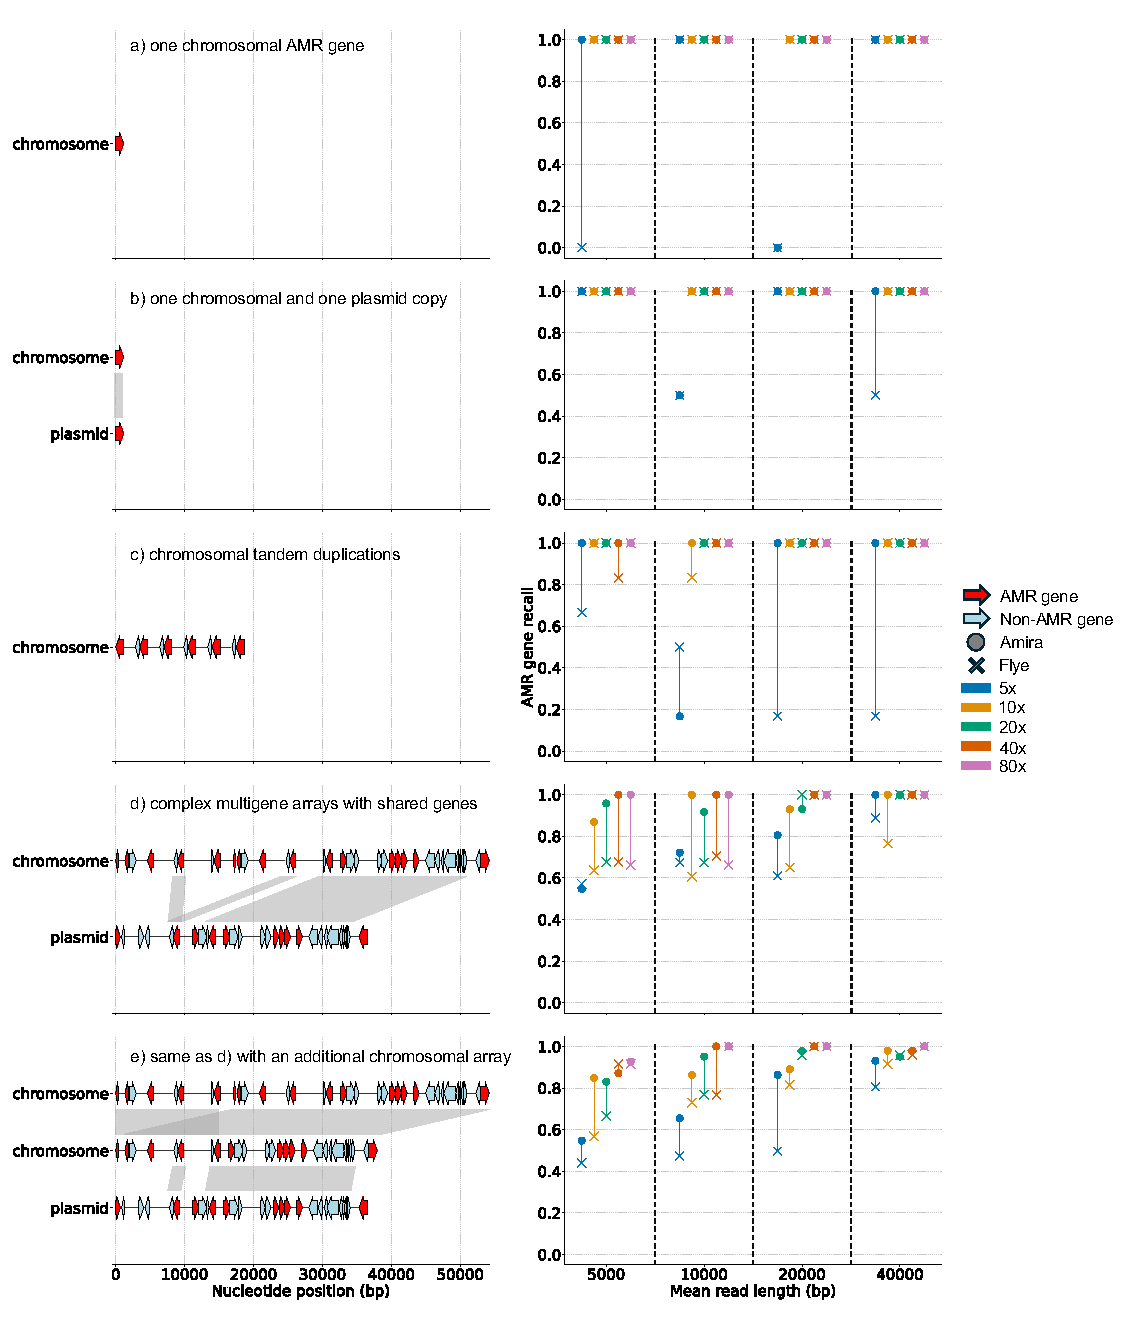
\includegraphics[width=1\linewidth]{Figures/figure_2.pdf}
\caption{Context plots detailing the AMR gene (red) and context gene (blue) content of five simulated scenarios (left) and the AMR gene recall of Amira and Flye with AMRFinderPlus applied to long reads simulated with Badread \cite{Wick2019} from each scenario (right). We artificially inserted each region into the chromosome or plasmid of an artificial \textit{E. coli} assembly containing no AMR genes, and applied Amira and Flye with AMRFinderPlus to the reads simulated from each simulated assembly. The x-axis of the left-hand plots shows the length of the inserted region in base pairs, and the y-axis shows which contig in the reference each region was inserted into. The x-axis of the right hand plots show the mean simulated read lengths (5 kb, 10 kb, 20 kb and 40 kb), the y-axis the recall for each genomic copy of an AMR gene. Each colour indicates the simulated read depth (5x, 10x, 20x, 40x or 80x).}
\label{fig:2}
\end{figure*}

\subsection*{Evaluation on empirical data}
\paragraph{}
Since simulations do not fully reflect the error profiles and AMR gene complexity of real long read sequencing data, we next evaluate how Amira performs on a dataset of 32 diverse \textit{E. coli} with Illumina and Nanopore reads available and known AMR gene content. Ten of these samples were sequenced using R10.4 Nanopore flow cells and 22 using R9.4.1. The evaluation samples span across the \textit{E. coli} phylogeny and are independent from those used to construct the reference panRG (Fig.\ref{suppfig:9}). The dataset contains 18 isolates with at least one multi-copy AMR gene, with one sample containing seven copies of a \textit{blaCMY} gene, of which six are in tandem. 
\paragraph{}
The mean read length across our evaluation set for the R9.4.1 samples is 14.2 kbp and Amira identified a mean of 11.9 genes per read. For the R10.4 samples, the mean read length is 4.7 kbp with 4.4 genes per read.
\paragraph{}
We compared the number and type of AMR genes found by Amira (using Nanopore data) to that pre-existing tools. The main comparator tools were AMRFinderPlus run on Nanopore-only assemblies generated with Flye \cite{Kolmogorov2019} (AMRFP Flye) and Raven \cite{10.1038/s43588-021-00073-4} (AMRFP Raven), hybrid assemblies generated with Unicycler \cite{Wick2017} (AMRFP Unicycler), and ResFinder \cite{Bortolaia2020}. AMR gene recall is defined similarly to the simulation evaluation. AMR gene precision is defined as the proportion of identified genomic copies of an AMR gene that were present in the truth assembly. Therefore, lower precision indicates a tool is over-estimating genomic copy number or calling genes that are absent from the truth assembly.
\paragraph{}
Amira achieved the highest recall on both R9.4.1 and R10.4 data, with 98.3\% and 98.5\% recall respectively, and precisions of 97.1\% and 99.5\% (Fig.\ref{fig:4}a). Notably, the results on R10.4 were achieved despite a much shorter mean read length than the reads in the R9.4.1 dataset. By contrast, the performance of the other tools varied by Nanopore flow cell technology. Flye had low recall (71.4\%) and high precision (100\%) for R9.4.1, but high recall (96.0\%) and precision (100\%) for R10.4. Unicycler had high recall (97.0\%) and precision (100\%) on R9.4.1 and low recall (89.2\%) with high precision (98.0\%) for R10.4. Resfinder had low recall on both datasets, with higher precision on the R9.4.1 samples (99.8\%) than the R10.4 samples (93.7\%) possibly due to incomplete de-multiplexing of the R10.4 samples following sequencing.
\paragraph{}
While we developed Amira specifically to better detect multi-copy genes, we found it excelled at detecting both single-copy and multi-copy genes in this dataset, with a mean per-gene recalls of 99.6\% and 98.9\% respecitvely (Fig.\ref{fig:4}d).
\paragraph{}
The accuracy of the nucleotide sequences for genes correctly called by Amira was consistently high for both the R9.4.1 and R10.4 datasets, with mean nucleotide identities of 99.9\% and 99.9\% respectively, compared to 98.4\% and 99.6\% for AMRFP Flye, 99.3\% and 99.6\% for AMRFP Raven, and 99.6\% and 99.6\% for AMRFP Unicycler (Fig.\ref{fig:4}c). Amira also used fewer computational resources than the assembly-based methods on this dataset, with a mean wall-clock time of 1,690 seconds (min 749, max 3,617) with a peak RAM of 6.0 GB (min 4.6, max 7.6) using 4 CPUs (Table.\ref{supptable:2}). 

\begin{figure*}
\centering
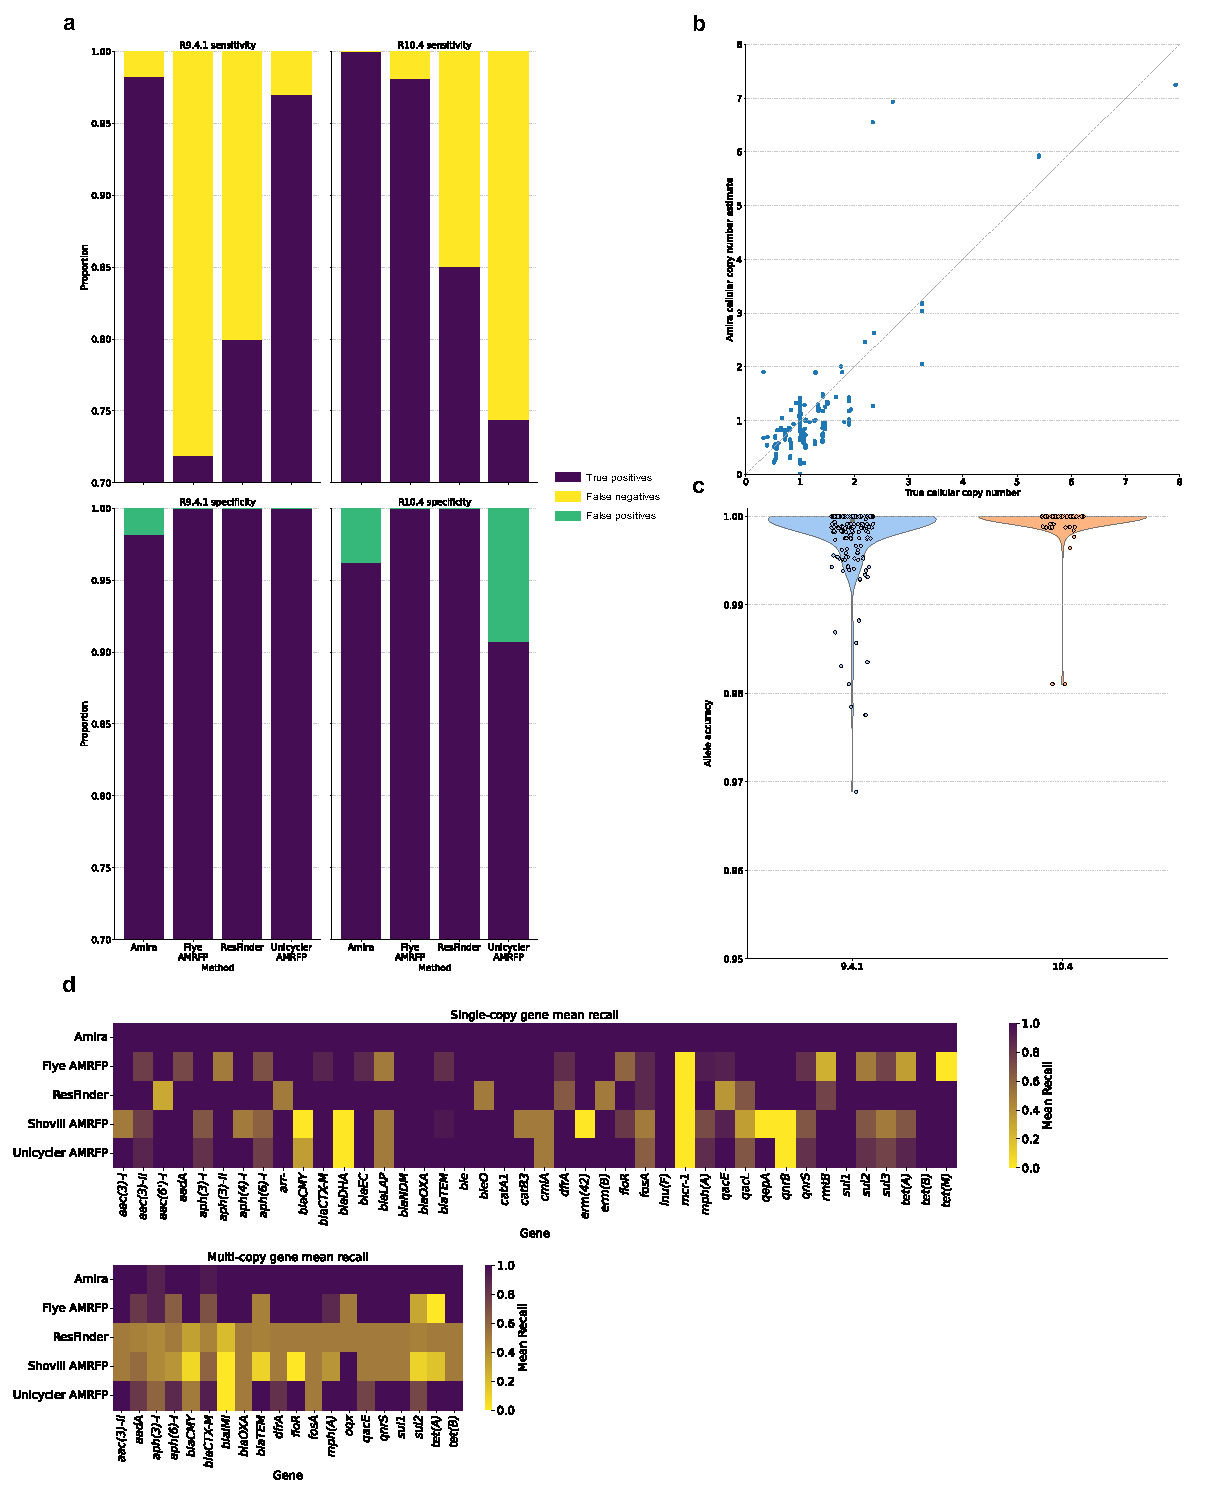
\includegraphics[width=1\linewidth]{Figures/figure_4.pdf}
\caption{(a) Recall and precision on the R9.4.1 and R10.4 samples. Note the axes run from 0.7 to 1.0. (b) Amira cellular copy estimates for each copy of each sample, compared to the true cellular copy number for the gene copy (estimated by dividing the mean Nanopore depth across the contig by the mean depth of the longest contig). (c) Gap-inclusive nucleotide similarities between the true nucleotide sequence for each each allele and that output by Amira or assembled by Nanopore-only assembly with Flye and Raven, and hybrid assembly with Unicycler. (d) Heatmaps showing the mean recall per method for each single and multi-copy AMR gene across the 32 test samples.}
\label{fig:4}
\end{figure*}

\subsection*{Genome assembly consistently underestimates AMR gene frequencies across bacterial populations}
\paragraph{}
After finding Amira better detects single copy AMR genes than assembly-based methods, we now apply Amira with to 8,525 \textit{E. coli} samples, 2,430 \textit{K. pneumoniae} and 410 \textit{E. faecium} with Nanopore reads available, and report the results of running AMRFinderPlus on assemblies for the same samples generated with Flye (AMRFP Flye). We report the recall of each method to detect at least one copy of each AMR gene with a read depth of at least 20\% of the mean read depth across the sample to prevent both methods from being penalized for not identifying low-depth AMR genes that may originate from contamination. The recall of Amira was consistently higher than that of AMRFP Flye across the three species. On the \textit{E. coli} dataset, the mean recall was 87.8\% (SD 20.8) for Amira and 55.2\% (SD 33.2) for AMRFP Flye (Fig. \ref{fig:5}a). For \textit{K. pneumoniae}, recall was 88.4\% (SD 21.8) vs. 65.6\% (SD 30.0) (Fig.\ref{fig:5}b), and for \textit{E. faecium}, 95.5\% (SD 14.0) vs. 57.2\% (SD 35.0) (Fig.\ref{fig:5}c). AMRFP Flye detected 24\%, 70\%, and 55\% of genes present in only one sample for \textit{E. coli}, \textit{K. pneumoniae}, and \textit{E. faecium}, respectively, compared to 90\%, 100\%, and 100\% for Amira.

\begin{figure*}
\centering
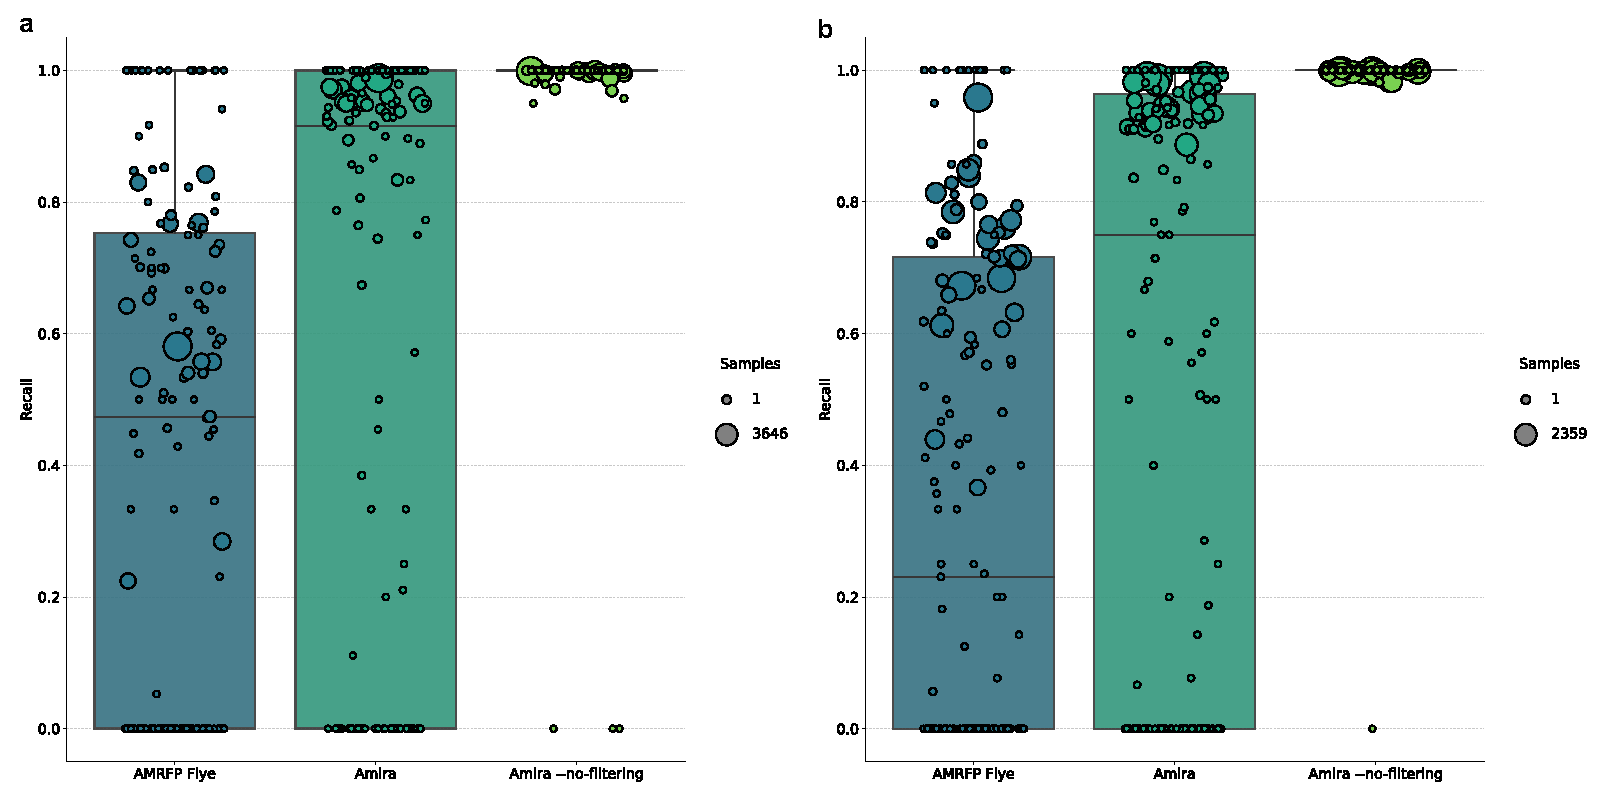
\includegraphics[width=1\linewidth]{Figures/figure_5.pdf}
\caption{Boxplots showing the per-AMR gene recall of Amira and AMRFinderPlus run on assemblies generated with Flye for 8,525 \textit{E. coli} (a), 2,430 \textit{K. pneumoniae} (b) and 410 \textit{E. faecium} (c) samples. Each point is a unique gene in the dataset. The y-axis indicates the recall of calling at least one copy of that gene, where recall is measured as the proportion of true samples each gene is identified in, with the truth defined from mapping the reads for each sample to a FASTA of reference AMR gene alleles. Point size scales with the number of samples that each gene is found in the truth.}
\label{fig:5}
\end{figure*}

\section*{Discussion}
\paragraph{}
Long-read sequencing technologies have substantially improved the quality and completeness of bacterial genome assemblies. However, assemblies generated from long read sequencing data are still susceptible to large-scale errors, particularly in regions associated with duplications that are mediated by mobile genetic elements. This can result in the underestimation of AMR gene content when using assembly-based AMR gene detection tools.
\paragraph{}
We developed Amira to address this challenge. Amira leverages the full length of long read sequences to differentiate multi-copy genes by their local genomic context. Through evaluation on simulated and curated truth datasets, we have demonstrated that Amira is more sensitive in detecting the presence and the number of copies of AMR genes than competing methods. This improvement is largely driven by use of the gene as the fundamental unit. By using Pandora \cite{pandora} to identify the genes on each sequencing read, Amira is robust to nucleotide-level SNP and INDEL errors, which are common in long-read sequences, as evidenced by the improvements in accuracy when applying Amira to datasets sequenced with error-prone R9.4.1 Nanopore reads. This allows the construction of significantly cleaner graphs that more accurately capture the underlying genomic structure than conventional \textit{k}-mer based methods, leading to better resolution of gene order and assignment of reads to the correct copy of each gene. We find this gives improved nucleotide-level accuracy compared to existing assembly- and read-based methods. 
\paragraph{}
Counter to our expectations, the improvement in recall, compared to assembler-based methods, is not solely due to multi-copy genes. Our interpretation is that this difference highlights the extent to which AMR gene detection from assembly is affected by contig breaks. AMRFinderPlus is able to report partially present genes however, users must manually distinguish genuinely fragmented genes and artefactual fragments caused by contig breaks or incomplete assembly of open reading frames. We estimated the impact of this difference on broad-scale surveillance of AMR gene prevalence, by applying Amira to the Nanopore reads of 8,525 \textit{E. coli}, 2,430 \textit{K. pneumoniae} and 410 \textit{E faecium}. Manual curation of assemblies at this scale is not feasible, so the true AMR genes present in each sample were defined prior to assembly. This confirms there is consistent under-detection of AMR gene content when using assembly-based approaches (Fig. \ref{fig:5}).
\paragraph{}
Simulations of progressively more challenging AMR gene arrays allowed evaluation of the relative effects of read length and depth and the intrinsic repeat structure of the genome. The recall of Amira and Flye improved with longer reads and greater sequencing depth, but we found that Amira was better able to leverage lower depth and shorter reads even in the most complex simulation scenarios.
\paragraph{}
Reference bias is a well documented challenge in bacterial variant-calling methods that rely on reference sequences, which arises when a single reference incompletely represents the diversity of a sample under analysis  \cite{pandora, 10.1016/s2666-52472100149-x, panaroo}. Soft reference bias refers to the impact on mapping of nucleotide divergence between the gene in the sample and that in the reference. Hard bias refers to entire regions (ie kb of sequence) from a sample which are missing from a reference, a consequence of the bacterial pan-genome. With Amira, we mitigate this by detecting genes from a pan-genome reference graph (panRG) constructed from a phylogenetically representative set of genomes of the species under analysis (and currently \textit{E coli}, \textit{K pneumoniae}, and \textit{E faecium}). In principle, if a sample has a multi-copy AMR gene that is flanked by rare genes not present in the panRG, the flanking genes will be invisible to Amira and it may not be possible to distinguish the reads corresponding to different copies of that AMR gene. By definition, this should be a rare occurrence. However, a more significant challenge is that the plasmid pan-genome in Enterobacteriaceae is extensive and there are over six million annotations in PLSDB \cite{10.1093/nar/gkab1111}. This far exceeds the number of genes that can be included in the panRG while maintaining acceptable memory and runtime performance. We address this by incorporating plasmid-specific genes from MOB-suite \cite{10.1099/mgen.0.000206} into the panRG to expand the context genes that can be detected. Although this is sufficient in our dataset, this is a limitation of our approach and a future improvement could involve expanding the panRG to include genes from plasmids with high abundance or of clinical concern. 
\paragraph{}
It is worth comparing this approach with that taken by wtdbg \cite{Ruan2020}. Wtdbg breaks reads into 256bp blocks, represents each block by its minimizers, and builds a “fuzzy-Bruijn graph” where equivalence-classes of these blocks are the alphabet. The blocks are all-by-all aligned in order to decide which are equivalent. As with our approach, wtdbg seeks to use a block-alphabet to simplify assembly. It has the advantage that it avoids reference-bias and can be run on any sample without a predefined pan-genome; however, it also has the disadvantages that the blocks are arbitrary, and that the block size may bear little relation to the repeats in the genome. By contrast, genes are broadly conserved in bacteria, and provide a reliable set of blocks to define chromosomal organisation, with the exception of a small set of genes that are frequently fragmented. The deeper differences lie in the details of the assembly methods: wtdbg uses standard approaches, cleaning its graph and popping bubbles before outputting contigs, whereas Amira uses paired suffix trees to enumerate the different contexts of AMR genes in all reads, and thereby separates out the different contexts they exist in.
\paragraph{}
Recent work has found evidence has found correlations between AMR gene dosage and MIC for specific gene-antimicrobial pairs \cite{10.1128/aac.02026-19, 10.1128/AAC.46.10.3334-3336.2002}. While MIC prediction was beyond the scope of this study, we anticipate that the more comprehensive identification of AMR gene content by Amira could enhance MIC prediction accuracy. Additionally, while Amira is designed to detect AMR genes, our approach could be directly applied to estimate the genomic and cellular copy numbers of any gene of interest through minor modifications.
\paragraph{}
Lastly, this work also introduces the gene \textit{de Bruijn} graph that was initially proposed in \cite{pandora}, a data structure that moves away from conventional \textit{k}-mers and is more robust to structural rearrangements that are frequent in bacteria. The gene DBG has the potential to be beneficial for a range of bioinformatic applications in place of \textit{k}-mers, particularly in bacterial genome assembly, and the approach can capture structural heterogeneity even at the level of single bacterial isolates. 

\section*{Methods}

\subsection*{Constructing species-specific panRGs}
\paragraph{}
Amira relies on Pandora \cite{pandora} to obtain an ordered list of gene identifiers, orientations and coordinates for each sequencing read using species-specific reference pan-genomes (abbreviated to panRGs). We developed a snakemake \cite{10.1093/bioinformatics/bts480} workflow to automate the construction of these panRGs from the annotations of a set of reference assemblies. This is supplemented with the annotations of 7,062 acquired AMR gene reference alleles from the NCBI Bacterial Antimicrobial Resistance Reference Gene Database (Accession PRJNA313047), and 4,056 plasmid-specific alleles used by MOB-suite \cite{10.1099/mgen.0.000206} to improve the representation of plasmid genes. The workflow begins by annotating the genes in the reference assemblies using bakta \texttt{v1.7.0} \cite{Schwengers2021}, supplements the annotations with the AMR and plasmid genes, then clusters the annotations into orthologs using Panaroo \texttt{v1.5.0} \cite{panaroo} with \texttt{--clean-mode sensitive --refind-mode off --remove-invalid-genes --length\_outlier\_support\_proportion 0.1 --merge\_paralogs --threshold 0.8 --len\_dif\_percent 0.0 -a pan}. All alleles less than 250 bp in length and all transposase or IS-related genes are then filtered, as these a significant source of inconsistent gene calls. After aligning the filtered clusters, we run make\_prg \texttt{v0.5.0} with default parameters, and construct a panRG using Pandora \cite{pandora} index \texttt{v0.12.0}, specifying \texttt{-k 15 -w 5}. 
\paragraph{}
For the reference assemblies for \textit{Escherchia coli}, we re-assembled the Illumina and Nanopore reads used in the 20-way analysis in \cite{pandora} with Hybracter \texttt{v0.7.3} \cite{Bouras2024} using default parameters. For \textit{Klebsiella pneumoniae}.... and for \textit{Enterococcus faecium} we .....

\subsection*{Constructing a read-coherent \textit{de Bruijn} graph in gene space}
\paragraph{}
Amira takes a FASTQ file of long reads as input, then uses Pandora to create a pseudo-SAM file that identifies the genes on each sequencing read. A hash table is created where the keys are read identifiers and values are an ordered list of gene identifiers, where the prefix of each gene identifier is the orientation of each gene relative to the orientation of the sequences of the gene in the panRG. A \textit{de Bruijn} graph is then constructed in gene space (referred to as a gene DBG) using the gene calls for each read. For each read of length $n$ that contains at least $k$ genes, a sliding window of size $k$ is moved across the list of genes in single-gene increments to generate $n - k + 1$ sub-lists, referred to as "gene-mers," that are analogous to \textit{k}-mers used in sequence assembly. The canonical representative for each gene-mer in a read is hashed and added as a node in a graph, where the canonical is defined as the lexicographically smaller of the gene-mer and its reverse complement. An edge is then added between each pair of adjacent gene-mers and it is annotated with the orientation of the target gene-mer relative to the canonical of the source gene-mer.

\subsection*{Correcting false paths in the graph}
\paragraph{}
There are two types of error we expect when mapping reads to the panRG with Pandora: complete failure to detect a gene or false positive detection. Gene detection can fail for two reasons. First, if a gene present in the reads of the sample under analysis is not present in the panRG, it cannot be detected. This may occur because none of the reference genomes used to construct the panRG contain rare genes found in the sample. These genes will be consistently absent across all reads, and contribute consistent paths to the gene DBG. Second, if sequencing errors ablate too many minimizers from a read, there may too few minimzers matching to the panRG to trigger gene detection. These errors are random and contribute erroneous paths to the graph that are low coverage, so can be removed. However, there are fewer potential minimizers to detect in short genes, so the impact of sequencing errors is larger. We address these up front, by setting a minimum length threshold on genes in our panRG of 250bp, and at run-time by applying low coverage cleaning thresholds to the graph. The second major error type is false positive detection of a gene. We found these occurred systematically at loci corresponding to fragmented partial genes, particularly transposases. The frequency of such fragments is presumably due to preference of mobile genetic elements to insert near other mobile genetic elements. We avoid the problem by removing transposases from our panRG. Amira uses several methods to account for the remaining errors, first applying correction to the graph itself, then using the corrected graph to correct the underlying list of genes of each sequencing read.
\paragraph{}
Following initial graph construction, all nodes that do not contain any reads with an AMR gene are pruned. All reads where >80\% of the nodes along the path followed by the read have a depth equal to one are then discarded. The gene DBG is reconstructed using the remaining reads, and an iterative correction algorithm is applied that consists of two stages: dead-end removal and path replacement. The dead end removal stage finds and removes all paths that start at a node with an in degree or an out degree of zero, end at a node with a degree greater than two and contain fewer than $k$ nodes in the path.
\paragraph{}
Path replacement begins by defining a set of candidate nodes that have an in or out degree greater than one. A depth-first-search is then conducted between all pairs of non-identical nodes, to obtain a set of all of paths with length $\leq 3k$. A reduced set of paths is defined by filtering out all paths that are wholly contained within another path. The filtered paths are sorted by length in descending order, and the paths clustered such that all paths in a cluster share a start and stop node. The clusters are processed in descending order of maximum path length within the cluster and for each cluster, the paths are sorted by descending mean node coverage. For each path $P_i$ with index $i$ in a cluster, we consider each lower coverage path $P_j$ with index $j$, where $j > i$, to be a potential false path. We extract the sets of nulceotide minimizers $M_i$ and $M_j$ from the reads for $P_i$ and $P_j$, respectively, using sourmash \texttt{v4.8.4} \cite{Pierce2019} with \textit{k}-mer size of 13 and scaled parameter of 10. Reads covering $P_j$ are corrected to follow $P_i$ if $\frac{|M_i \cap M_j|}{|M_i|} \geq 0.8 \quad$ or $\quad \frac{|M_i \cap M_j|}{|M_j|} \geq 0.8$.

\subsection*{Assigning reads to paths}
\paragraph{}

For each copy of each AMR gene in a bacterial sample, there exists a minimum length path through the corrected gene DBG that incorporates a sufficient number of context genes to make it distinct. When the genomic context immediately flanking each copy of a multi-copy AMR gene differs, only one context gene is needed. However, in cases where the number of genes within a duplicated genomic region (that contains an AMR gene) significantly exceeds the value of $k$, it is necessary to leverage the full read length to differentiate the paths. For each unique AMR gene identified by Pandora, this is addressed by first clustering reads by the presence of blocks of contiguous nodes that contain an AMR gene (referred to as internal blocks), then sub-clustering the reads by the paths of nodes external to each internal block (referred to as external blocks). To facilitate this, we begin by constructing a generalised suffix tree, where each "letter" represents a node identifier, and each "word" corresponds to the ordered list of node identifiers for the path followed by a read through the gene DBG. Each read contributes two words to the suffix tree: one for its forward orientation and the other for its reverse. This is referred to as $T_p$.

\paragraph{}
Internal blocks are defined for each unique AMR gene $g$ in the first round of clustering. Firstly, the reads containing $g$ are identified and the set of anchor nodes $A$ is determined using the reads. Anchor nodes indicate the start and end points of internal blocks and they are read-dependent; a node may be an anchor in one read, but occur within an internal block in another. In fact, internal blocks may be nested and a shorter block may be entirely contained within a longer block but correspond to a distinct full length path. A node is defined as an anchor node if it contains $g$, and either appears adjacent (in any read) to a node that does not contain $g$, or occurs at the terminal end of a read in $\ge$60\% of reads that contain the node. Every anchor node $a_i$ is queried in $T_p$ to obtain all the sub-lists of nodes downstream of $a_i$, and a secondary suffix tree $T_s$ is constructed from the reverse of the suffixes (Fig.\ref{fig:6}b). Every other anchor node $a_j$ is queried in $T_s$, such that $a_i \neq a_j$, to collect and cluster reads by the longest internal block they contain.
\paragraph{}
After identifying the set of internal blocks $B$ for $g$, the paths of nodes external to each internal block $b_i$ are used to differentiate long duplicated regions with paths that are followed by the reads and diverge outside of $b_i$. This is achieved by querying $T_p$ for $b_i$ and tracking the suffixes downstream of $b_i$, exclusive. Simultaneously, the reverse of $b_i$ is queried in $T_p$ and the reverse of the suffixes obtained is stored as upstream external blocks, again excluding $b_i$. This creates two sets for $b_i$: one corresponding to the external blocks upstream ($U_i$) of $b_i$, and one to the downstream external blocks ($D_i$). A clustering approach is applied to $U_i$ and $D_i$ that infers the number and full length of the unique underlying paths supported by each external block. This sorts $U_i$ and $D_i$ by descending path length and clusters blocks together that are fully contained within a longer clustered external block, skipping blocks that are sub-blocks of the longest block in more than one cluster. Subsequently, the shortest external block in each cluster is selected as the representative for the underlying path. For each $b_i$, a minimum-length node-space path is inferred by joining any cluster representative of $U_i$, $b_i$, and cluster representative of $D_i$ if they all share at least one read, and paths are filtered out if they are sub-paths of any longer path (Fig.\ref{fig:6}c). The number of context genes necessary to differentiate the paths is minimized by first converting each node-space path into gene-space ($P_i$). All possible sub-paths of $P_i$ of any length are enumerated, and any sub-path filtered out if it is a sub-path of any other path $P_j$, where $P_i \neq P_j$, or does not contain the same number of copies of $g$ as $P_i$, and the sub-path that is covered by the most reads is selected as the final path (Fig.\ref{fig:6}d). Finally, all reads that contain each final path are collected using $T_p$ and two FASTQ files are generated: one file stores the full sequences of all reads containing the path, enabling estimation of the cellular copy number of the path; the other file stores the nucleotide sequences corresponding to each AMR gene copy in the path.

\begin{figure*}
\centering
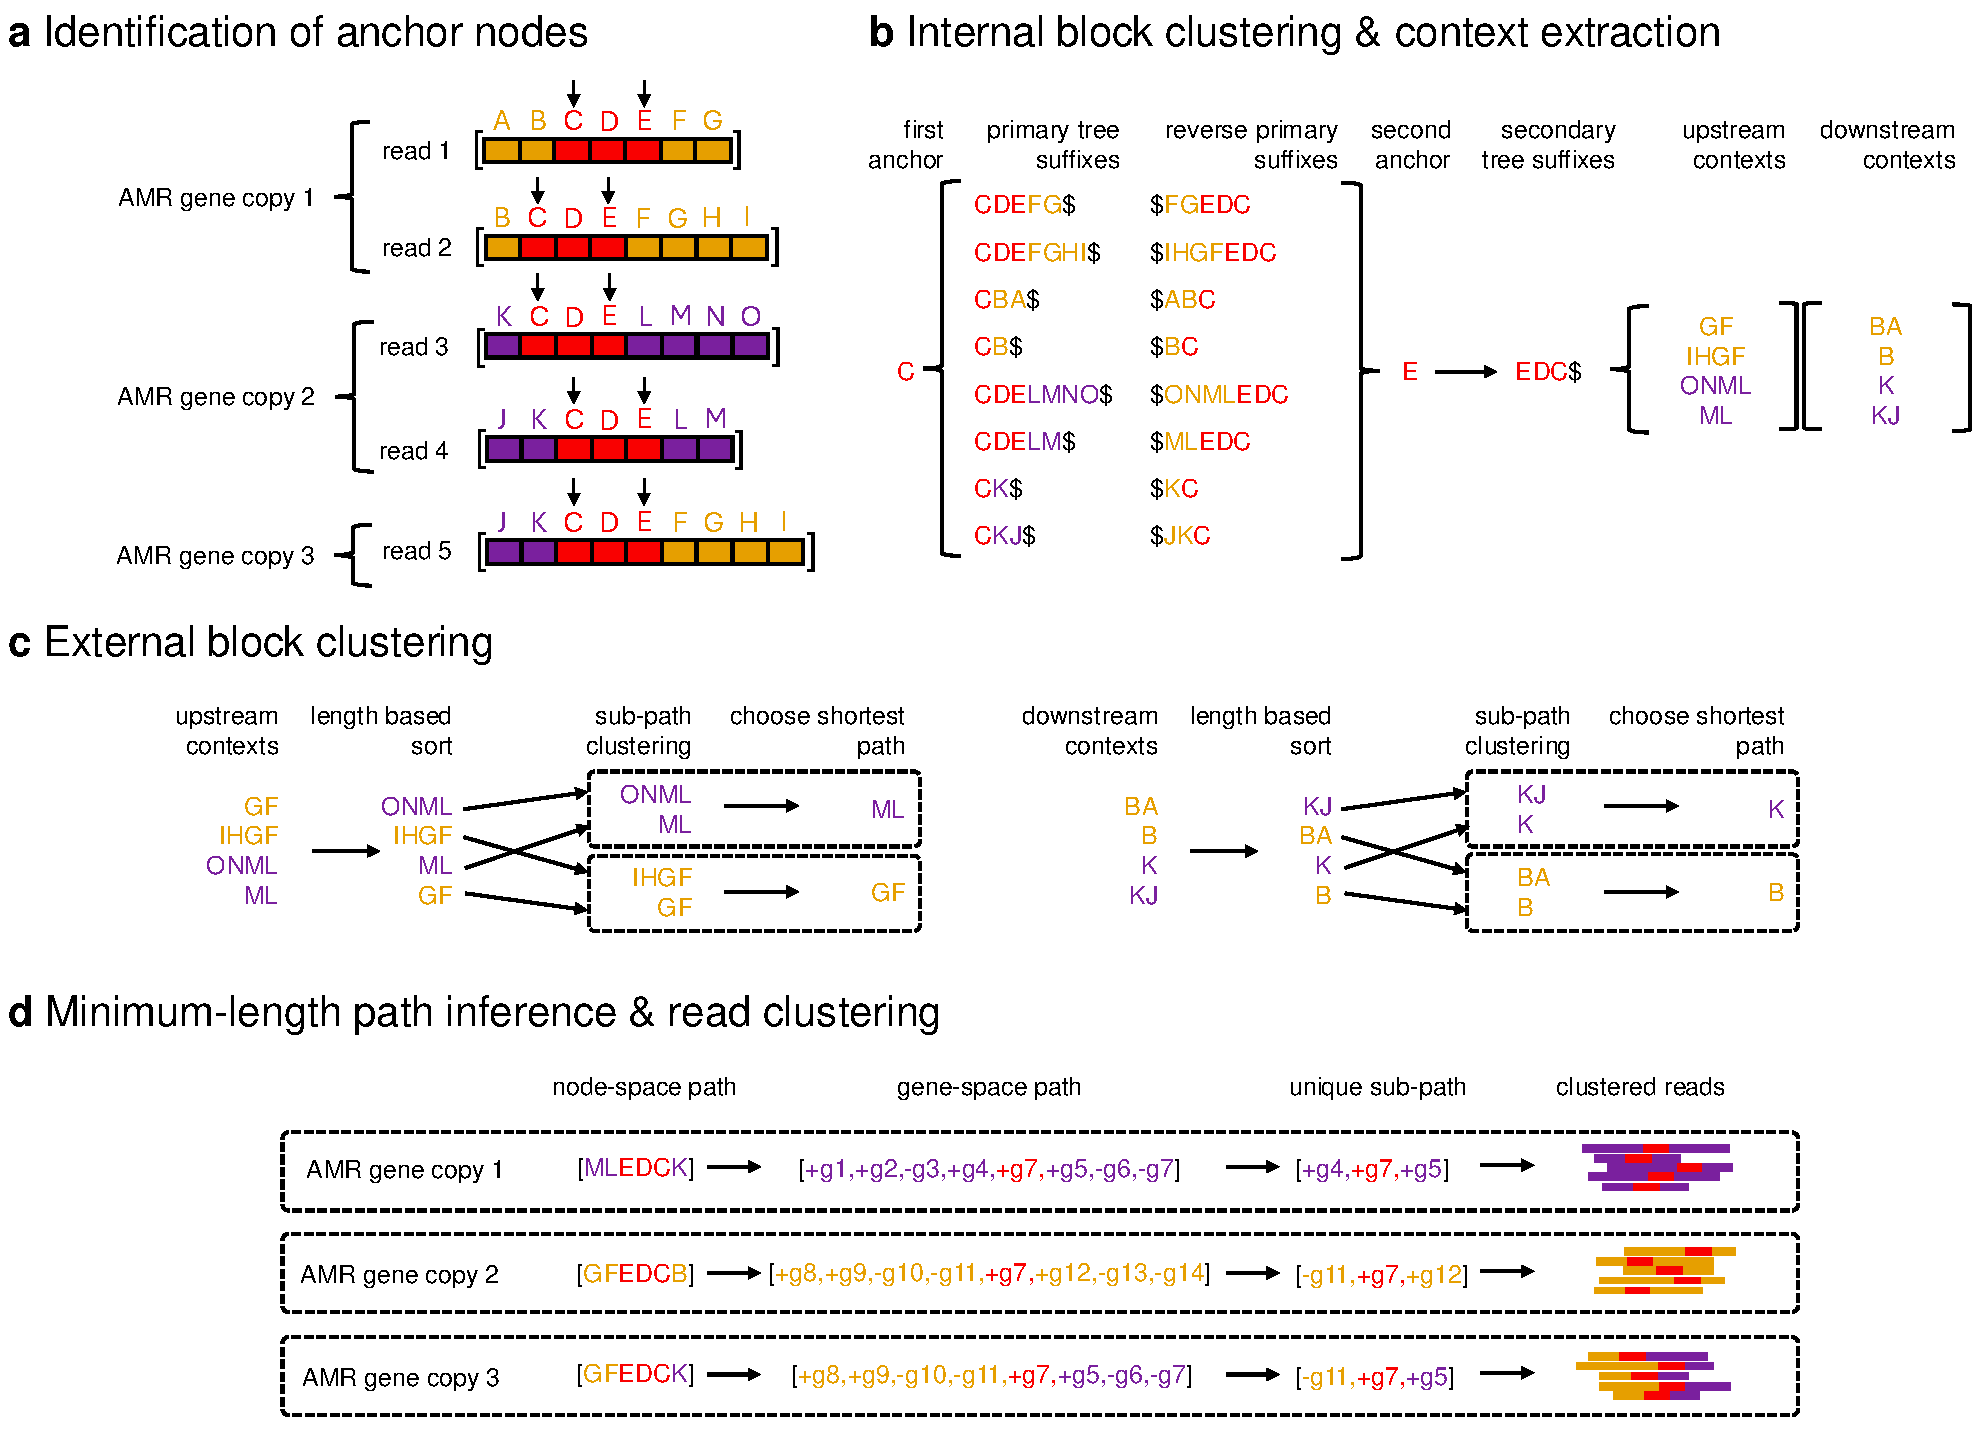
\includegraphics[width=1\linewidth]{Figures/figure_6.pdf}
\caption{The approach used by Amira to separate the reads containing multi-copy AMR genes using paths through the corrected gene DBG. (a) The set of “anchor” nodes are identified for each unique AMR gene. These are nodes containing the AMR gene that occur immediately adjacent to any node not containing the AMR gene in any read. (b) Internal blocks are defined between pairs of anchor nodes. This process begins by identifying the suffixes of the first anchor by querying a suffix tree built from the list of node identifiers for each read. Next, the second anchor node is queried in a second suffix tree constructed from the reverse of the suffixes obtained in the initial search. The blocks of nodes external to each internal block are then obtained. (c) External blocks are clustered into underlying paths. Blocks are sorted from longest to shortest, and clustered with a longer block if they are entirely contained within it. Blocks that belong to multiple clusters are disregarded and the shortest block within each cluster is selected as the representative. (d) Minimum-length paths that differentiate AMR gene copies are inferred and reads are clustered by the presence of these paths. Full-length paths in node space are determined by joining external and internal blocks that share at least one read, then converted to gene-space paths. For each gene-space path, all sub-paths are enumerated and the single sub-path that is not a sub-path of any other gene-space path, contains the same number of AMR genes as the full length path and is covered by the most reads is chosen as the minimum-length path. Reads are clustered based on the presence of the minimum-length paths.}
\label{fig:6}
\end{figure*}

\subsection*{Estimating the cellular copy number of each AMR gene copy}
\paragraph{}
The cellular copy number of each genomic copy of every previously identified AMR gene is estimated using relative \textit{k}-mer counts, to account for multi-copy plasmids with identical gene content. The frequencies of all \textit{k}-mers (with $k$ = 15) in the sample’s FASTQ file are computed using Jellyfish \texttt{v2.3.0} \cite{10.1093/bioinformatics/btr011} and a probabilistic mixture model proposed by \cite{10.1101/gr.279449.124} is used to identify a cut-off separating erroneous from true \textit{k}-mers. Briefly, a log-likelihood function is defined over the \textit{k}-mer frequency spectrum, modeling the probability of each observed count $i$ as:

\[
P(i) = w \cdot \frac{e^{-1} \cdot 1^i}{i!}  + (1 - w) \cdot \frac{e^{-c} \cdot c^i}{i!}
\]

Where $w$ is the proportion of erroneous \textit{k}-mers, following a Poisson distribution with mean $\lambda = 1$, and $1-w$ is the proportion of correct \textit{k}-mers, assumed to follow a Poisson distribution with mean $\lambda = c$. The parameters $w$ and $c$ are optimised using the L-BFGS-B algorithm implemented in Scipy \texttt{v1.12.0} \cite{2020SciPy-NMeth}, with bounds $0 \le w \le 1$ and $c \ge 1 \times 10^{-5}$. The \textit{k}-mer count cut-off is then selected as the smallest integer $i$ where the probability of a \textit{k}-mer originating from the fraction of correct \textit{k}-mers is greater than the error fraction. All \textit{k}-mers with counts below this cut-off are discarded. Next, the filtered \textit{k}-mer count histogram is smoothed using a Savitzky–Golay filter (window length = 30, polynomial order = 3) and the mean read depth is estimated as the count corresponding to the highest peak in the smoothed histogram. Finally, for the minimum-length path of each genomic copy of the AMR genes identified earlier, the filtered histogram is used to compute the median \textit{k}-mer count across all \textit{k}-mers that intersect with the path. This value is divided by the product of the estimated mean read depth and the number of copies of the specific AMR gene within the path to obtain an estimate for the cellular copy number.

\subsection*{Obtaining AMR gene alleles}
\paragraph{}
The final step is to obtain the allelic sequences of each AMR gene genomic copy. Minimap2 \texttt{v2.17} \cite{10.1093/bioinformatics/bty191} is used to map the FASTQ file of the nucleotide sequences of each AMR gene copy to all reference alleles that are contained in the cluster of orthologous genes in the panRG for that AMR gene. The reference allele that most closely matches the reads in the FASTQ with identity $\ge$90\% and coverage $\ge$90\% by default is selected, and five iterations of polishing using racon \texttt{v1.5.0} \cite{10.1101/gr.214270.116} is conducted to obtain the final sequence of each AMR gene copy.

\subsection*{Evaluating on simulated data}
\paragraph{}
We developed a snakemake \cite{10.1093/bioinformatics/bts480} workflow to simulate \textit{E. coli} samples with varying complexities in AMR gene content to assess the accuracy of Amira gene calling and its correlation with read depth and length. A synthetic assembly was generated using the \textit{E. coli K-12} reference sequence (Accession \textit{NC\_000913.3}) after removing a single copy of \textit{blaEC} at positions 4377811-4378944, and a \textit{ATCC 11775} reference plasmid (Accession \textit{CP033091.2}) that contains no AMR genes. The workflow inserts complex AMR regions identified from the literature into the sythetic assembly, then simulates sequencing read sets for input into Amira using badread \texttt{v0.4.1} \cite{Wick2019}, with parameters \texttt{--error\_model "Nanopore2023"} and all combinations of: \texttt{--quantity “10x”, “20x”, “40x”, “80x”} and \texttt{--length “5000,6615.5”, "10000,10815.5", "20000,19215.5", "40000,36015.5"}. Reads were simulated using just the backbone chromosome and plasmid as a negative control, and five additional test cases were simulated using increasingly complex AMR gene containing regions that were identified from public datasets. We compared the genomic copy number recall of Amira \texttt{v0.8.0} to Flye \texttt{v2.9.3} with AMRFinderPlus \texttt{v3.12.8} \cite{Feldgarden2021} with database \texttt{v2024-01-31.1} and options \texttt{--plus --organism Escherichia}. Genes with “PARTIALX” or “PARTIALP” in the “Method” column of the AMRFinderPlus output were excluded.

\subsection*{Evaluating on empirical data}
\paragraph{}
The Nanopore and Illumina reads for 32 \textit{E.coli} isolates in supplementary table \ref{supptable:1} were retrieved for the empirical evaluation. Ten of the samples were sequenced using R10.4 flow cells (referred to as the R10.4 samples) and 22 using R9.4.1 flow cells (referred to as the R9.4.1 samples). The publicly available RefSeq assemblies for the R9.4.1 samples were also retrieved to define the true AMR gene content for these samples. For the ten R10.4 samples, Trycycler v…. Was used to generate consensus assemblies from individual assemblies using Flye? V…, Unicycler? V… hybrid and …. The Illumina and Nanopore reads were mapped to the Trycycler and RefSeq assemblies using minimap2 \texttt{v2.28} \cite{10.1093/bioinformatics/bty191} with options \texttt{--eqx -a -x sr --secondary=no} for the Illumina reads, and \texttt{--eqx -a -x map-ont --secondary=no} for the Nanopore reads. The Nanopore read depths across each assembly were visualised, normalised by the mean read depth for each contig containing an AMR gene, to check for regions of elevated coverage that may indicate collapsed duplications, that were present in two samples. The reads mapping to the problematic contigs were subsetted with samtools \texttt{v1.17} \cite{Li2009} and pyfastaq \texttt{v3.17.0} and reassembled using Canu v2.3 \cite{Koren2017} with \texttt{genomeSize=20k}. One round of short-read polishing was then conduced for each with polypolish v0.6.0 \cite{10.1099/mgen.0.001254}. TNA \texttt{v0.3.0} \cite{TNA} was used to visualise the alignments of the reassembled contigs to the reference. Further information detailing the assembly validation be found in figures \ref{suppfig:1}-\ref{suppfig:6}.
\paragraph{}
A true AMR gene in the truth assemblies is defined as any sequence present in the assembly that is at least 90\% identical and 90\% covered by a reference allele that is included in the panRG. This was done by mapping all the AMR gene reference alleles included in the reference panRG to each assembly using minimap2. All hits with alignment coverage <90\% and identity <90\% were filtered and the remaining hits were sorted first by identity, then by length. The best match was chosen in cases where multiple alleles overlapped with each other. False pseudogenes are frequent in bacterial assemblies \cite{Cooley2024} and this relaxed coverage threshold avoids penalisation of AMR genes that are present in the truth assemblies but base-level errors are causing frameshift or premature stop codon errors within open reading frames. All of the tools tested call AMR genes that are less than 100\% covered by a reference. 
\paragraph{}
The Nanopore read sets for each sample was subsampled to 200x using rasusa \texttt{v2.1.0} \cite{Hall2022} and the accuracy of Amira \texttt{v0.8.0} was compared to that of AMRFinderPlus \texttt{v3.12.8} \cite{Feldgarden2021}, with database \texttt{v2024-01-31.1} and options \texttt{--plus --organism Escherichia}, run on Nanopore-only assemblies generated with Flye \texttt{v2.9.3} \cite{Kolmogorov2019} and Raven \texttt{v1.8.3} \cite{10.1038/s43588-021-00073-4}, and hybrid assemblies generated with Unicycler \texttt{v0.5.0} \cite{Wick2017}. All assemblers were run using their default parameters and genes with “PARTIALX” or “PARTIALP” in the “Method” column of the AMRFinderPlus output were excluded. Resfinder \cite{Bortolaia2020} \texttt{v4.6.0} was also ran on the Nanopore reads for each sample with options \texttt{-s e.coli -acq --Nanopore} by generating an index of all AMR alleles in our reference panRG using kma\_index \texttt{v1.4.15} \cite{Clausen2018}. All ResFinder hits with <90\% identity or <90\% coverage were excluded. The true cellular copy numbers of each genomic copy of an AMR gene were estimated by obtaining the mean Nanopore read depth across the contig for the gene, normalised by the mean read depth across the longest contig in each sample. All alleles for each unique AMR gene present in both the reference assembly and the output of the evaluated tool were aligned using MAFFT \texttt{v7.526} \cite{mafft} and option \texttt{–auto}. Nucleotide-level accuracies were calculated as the proportion of matching columns in the alignment between each reference allele and the output allele. Each output allele was matched to the closest reference allele without replacement, prioritising nucleotide accuracy followed by the absolute difference in cellular copy number. 
\paragraph{}
Divergent paths in a single connected component of the Amira graph were resulting in false positive gene calls in one sample. By subsetting the reads unique to the differing paths and visualising the pileups with IGV \texttt{v2.19.1} \cite{10.1093/bib/bbs017}, this was found to be the result of the presence of a minor frequency structural variants of a plasmid in this sample (Fig.\ref{suppfig:8}). We chose not to penalise the assemblers for missing the low-frequency variant, nor penalise Amira for identifying it as it resulted from genuine heterogeneity present in the read sets.

\subsection*{Estimating AMR gene frequencies across large datasets of long read sequences}
\paragraph{}
Following evaluation of Amira on simulated scenarios and a curated truth dataset, we next use Amira to analyse 8,525 \textit{E. coli}, 2,430 \textit{K. pneumoniae} and  410 \textit{E. faecium} samples in the ENA with long reads available. A TSV of all run accessions for Tax Id 562 for \textit{E. coli}, Tax Id 563 for \textit{K. pneumoniae} and Tax Id 1352 for \textit{E. faecium} (as of 11 February 2025) was obtained from the ENA, and all read sets downloaded if they contained the terms “Nanopore”, “MinION”, “PromethION” or “PacBio” in the “description column of the TSVs. Amira \textit{v0.8.0} was then ran with default parameters, as was AMRFinderPlus \texttt{v3.12.8} with options \texttt{–plus –organism Escherichia}, \texttt{Klebsiella\_pneumoniae} or \texttt{Enterococcus\_faecium} on long read-only assemblies generated with Flye \texttt{v2.9.3} with default parameters. The true AMR genes per sample were determined by first mapping the long reads to a FASTA of the AMR gene alleles in the panRG. The mean read depth of the sample was estimated by mapping the reads to a FASTA of core genes for the species with minimap2 with option \texttt{-x map-ont} and using samtools \texttt{coverage}. The number of reads aligned to each AMR gene allele with $\geq$90\% alignment coverage and $\geq$90\% identity were counted and a gene reported as present if the number of reads that satisfy this criteria was at least 20\% of the mean read depth across core genes. Samples where Amira and Flye did not complete within 240 minutes, samples that failed to run for either tool and genes with a value of <90\% in the “\% Coverage of reference sequence” column of the AMRFinderPlus output were excluded.

\subsection*{Data and code availability}
\paragraph{}
Amira is freely available from \url{https://github.com/Danderson123/Amira} under an Apache-2.0 license and can be installed via PyPI or Singularity \cite{10.1371/journal.pone.0177459}. The panRG construction pipeline is available from \url{https://github.com/Danderson123/Amira_panRG_pipeline}. Snakemake workflows to rerun the analyses in this paper and the long read accessions for the samples used in the ENA evaluation are available at \url{https://github.com/Danderson123/amira_paper}. The \textit{E. coli} panRG is available from \url{https://drive.google.com/file/d/13c_bUXnBEs9iEPPobou7-xEgkz_t08YP/view?usp=sharing}, the \textit{K. pneumoniae} panRG is available from \url{https://drive.google.com/file/d/1DYG3QW3nrQfSckIX9Vjbhbqz5bRd9W3j/view?usp=drive_link} and the \textit{E. faecium} panRG is available from \url{https://drive.google.com/file/d/1AzzFNRbH6VXPj5CX2txlcxhW8AhL9HSh/view?usp=sharing}. The the long reads, short reads and reference assemblies for all of the empirical evaluation samples are available via figshare and the accession can be found in table \ref{supptable:1}.

\section*{Acknowledgements}
\paragraph{}
The authors are very grateful to Martin Hunt, Leah Roberts and Wei Shen for critical review of the manuscript, William Matlock for guidance on MIC prediction, and John Lees, Julian Parkhill and Nassos Typas for their valuable advice, guidance and support throughout the project as part of the thesis advisory committee for DA. We also thank Daria Frolova and Samuel Horsfield for their general interest and providing fruitful discussion during the undertaking of this work.

\section*{Contributions}
\paragraph{}
Conceptualization: D.A., Z.I. Data Curation: D.A, T.L., R.W., L.J. Formal analysis: D.A. Funding acquisition: Z.I. Investigation: D.A. Methodology: D.A., L.L, Z.I. Project administration: Z.I. Resources: R.W., L.J., Z.I. Software: D.A. Supervision: Z.I. Validation: D.A. Visualisation: D.A. Writing – original draft: D.A., R.W., Z.I. Writing – review \& editing: D.A., Z.I.

\section*{Bibliography}
\bibliographystyle{bxv_abbrvnat}
\bibliography{refs.bib}